% 1988 年广东卷文史类第二卷第二题：四棱锥 P-ABCD
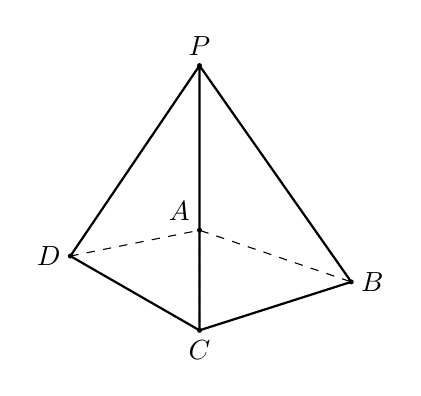
\begin{tikzpicture}[scale=0.82,>=stealth]
  \coordinate (P) at (2.0,4.1);
  \coordinate (D) at (0,1.15);
  \coordinate (C) at (2.0,0);
  \coordinate (B) at (4.35,0.75);
  \coordinate (A) at (2.0,1.55);
  \draw[thick] (P)--(D) (P)--(C) (P)--(B);
  \draw[dashed] (P)--(A);
  \draw[thick] (D)--(C)--(B);
  \draw[dashed] (D)--(A)--(B) (A)--(C);
  \fill (P) circle (1.1pt) node[above] {$P$};
  \fill (A) circle (1.1pt) node[above left] {$A$};
  \fill (B) circle (1.1pt) node[right] {$B$};
  \fill (C) circle (1.1pt) node[below] {$C$};
  \fill (D) circle (1.1pt) node[left] {$D$};
\end{tikzpicture}
